\documentclass[10 pt]{article}

\usepackage{fontspec}
\defaultfontfeatures{Mapping=tex-text}
\setmainfont{Minion Pro}

%\usepackage{graphicx}
%\usepackage{fullpage}

\usepackage{lastpage, fancyhdr}
\pagestyle{fancy}
\lhead{Scott O'Connor}
\chead{Phil 234} 
\rhead{\emph{Meno}}
\lfoot{}
\cfoot{\thepage\space of \pageref{LastPage}} 
\rfoot{}

\thispagestyle{empty}


\begin{document}
\author{Phil 234}
\title{\emph{Meno}}
\maketitle

\section*{Overview}
The dialog begins with (M)eno, a Thessalian, asking (S)crates whether virtue is teachable (70a1-4). M is politically ambitious, young, handsome, well-born, and visiting Athens with Anytus, one of S's prosecutors, as a host.  M will embark on a controversial military and political career that ends with his young death by the Persian king.  

`Virtue' translates `arete', but translation of this Greek word is difficult. The difficulty is best introduced by analogy. There is a difference between the excellent and mediocre boxer, the excellent and mediocre ice-skater, the excellent and mediocre university student, etc. The Greeks believed that just as you could excel in some specific activity, you could excel at being human. They thought there was a difference between being an excellent human and being a mediocre human. `Arete' is here used to describe the excellence of excellent human beings. `Virtue' was its standard translation, but that was complicated when `virtue' becomes restricted to set of moral qualities that included chastity, temperance, etc.

Virtue was important to the Greeks. They dedicated their time and resources to attain it, and they placed a very high value on its teachability. They cared not merely to live, but to become and be excellent humans. Famous poets, speakers, politicians, generals, etc., claimed they could teach virtue; students and their families paid hefty sums for the education. So to ask whether virtue is teachable, as M asks S, is a very controversial question. Answering `no' is risky.  Three options for the acquisition of virtue are discussed: 
\begin{enumerate}
\item You are born with it. 
\item You acquire it through practicing it. 
\item You acquire it through education, i.e., one person teaching that knowledge to you. 
\end{enumerate}
Which one will Socrates ultimately argue for? 

As well as answering that question, our primary interest is M's challenge that inquiry into the nature of things is impossible. S's response will teach us two things: 1) S's epistemology, most especially the difference between knowledge and belief (opinion), and 2) how S believes that he can inquire into, and help others inquire into, the nature of those things he does not yet know. 


\section*{Socrates' Challenge}

S claims that he does not know whether virtue can be taught because he does not know what it is (71b1--8). So, we must first answer the question `what is virtue?' before we can determine whether virtue is teachable. Recall that an answer to such a question is called a Socratic Definition. S, therefore, is here assuming the following principle: 
\begin{description}
\item[The priority of definition:] In order to know what qualities X possesses, you must know what X is, i.e., you must know the Socratic definition of X. 
\end{itemize}
This principle rests on two further claims: 
\begin{enumerate}
\item There is a distinction between essential and non-essential features, e.g., humans are essentially rational, but they are not essentially capable of laughter.
\item Essential features are explanatory of (some) non-essential features.
\end{enumerate}
Since S does not know the essence of virtue, he does not know what follows on from that essence, including whether it is teachable. But we might question S here: he claims that to know whether M is good-looking, rich, or well-born, you must know who M is.  If you do not know at all who M is, then you cannot know what qualities belong to M. This seems implausible. Suppose I see a red-haired stranger. Can I not know that the person has red hair without knowing who they are? S might respond by asking what we mean by saying that we know that the person has red hair. Assume that the person's name is John. If I do now know who John is, then S will claim that I cannot know that John has red hair just by looking at the person in the room. I can know, perhaps, that there is a person in a room with red hair. But that is quite different from knowing that \emph{John has red hair}. Since I don't know that the person is John, I couldn't know that John has red hair. 

The dialog proceeds by discussing  various candidate definitions of virtue. During this initial discussion, S again illustrates the requirements for a Socratic definition. He does so in two ways. He first has M to try define virtue and illustrates the requirements by failure. He then gives a few successful definitions of color. This tells M how he should define virtue. Recall that an adequate definition must be a) general, b) univocal, and c) explanatory.  

\section*{The paradox of inquiry}
M grows frustrated with S's demands for a definition and argues that we cannot inquire into the definition of something if we are in a complete blank regarding that thing (80d5-80e5):

\begin{enumerate}
\item[P1.] If you know X already, you cannot inquire into X. 
\begin{itemize}
\item Read `inquire into X' as `inquire after the definition of X'. 
\item When people begin searching for something, they do not yet possess what they are searching for. So if they did already possess something, it makes no sense to search for it.
\end{itemize}
\item[P2.] If you do not know X, you cannot inquire into X (since you don't know what to search for).
\begin{enumerate}
\item If you do not know \emph{at all} what X is, then you cannot start to inquire into X...you will not know how to start even looking.
\item If you do not know \emph{at all} what X is, and if you stumble upon X, you will not know that what you stumbled upon is X, e.g., if you do not know who M is, but stumble upon him, then you will not know that the person you stumbled upon is M. 
\end{enumerate}
\item[P3.] Either you know X or you do not know X. (Implicit Premise) 
\item[C.] Therefore you cannot inquire into X.
\end{enumerate}
Impasse!  S claimed that we cannot find out whether virtue is teachable until we know what virtue is, i.e., know the essence of virtue.  But M argues that we cannot inquire into the essence of virtue if we know nothing at all about it. This is a serious impasses. It seems we must know at least something about virtue before we can investigate its nature. But it also seems that we cannot know anything about virtue without already knowing its nature. So, it follows that it is impossible to find out whether virtue is teachable. 

\section*{The Theory of Recollection (TR)}
To solve the dilemma, S must feasibly reject at least one of the premises. It is difficult to identify which one. His core claim is that ``what we call learning is recollecting things we already know (81b3--c9).'' This is called \emph{The Theory of Recollection (TR)} because it claims that learning is merely recollecting what one used to know but subsequently forgot. 

In order to defend TR, S engages with one of M's slaves. S's goal is to show that the slave can learn something by recollection, i.e., he learns/recollects the lengths of each side of a 8 sq ft square (85d2-10). Before we look at the details, consider how this might solve the paradox. S seems to distinguish between latently knowing and explicitly knowing something. He subsequently endorses these two claims:  

\begin{enumerate}
\item We cannot inquire into what we \emph{explicitly} know, but \emph{we can} inquire into what we \emph{latently} know. 
\item We cannot inquire into what we do not even \emph{latently} know, but \emph{we can} inquire into what we do not \emph{explicitly} know.
\end{enumerate}



\noindent S's proof that the slave can learn through recollection:

\begin{itemize}
\item The slave gives correct answers to certain questions about geometry.
\begin{itemize}
\item S uses his Socratic method---he asks misleading questions sometimes; he gets the slave to claim knowledge and then to confess \emph{puzzlement}; thereafter the slave gets it right by applying his own reasoning, not by bowing to S's authority.
\end{itemize}
\item If the slave can give correct answers, he must, in some sense, know the answers. 
\item The slave has not learned geometry before. 
\item The slave was not taught any geometry by S in their exchange--so the slave didn't \emph{learn} it then either.
\begin{itemize}
\item Since S does not himself have the answers, he cannot be teaching them to the slave. 
\item S claims that his questions merely elicit the slave's opinions. 
\end{itemize}
\item We need some explanation of why the slave, through his discussion with S, will reliably \emph{reject} false beliefs and \emph{accept} true beliefs. 
\item S claims that this is possible because the slave (like everyone) once knew (in a disembodied state) but forgot, and hence can recognize the truth, and so reject the false.
\item S claims that the slave \emph{will} know it through further questioning
\end{itemize}
 
Two points to note along the way: 

1. S emphasizes that he does not tell the answer to the student. If he teaches at all, he does not teach by any direct transfer of knowledge. The student does not come to think that x is P because S says that x is P. Can we think of any other form of education where there is no real direct transfer of knowledge? 


%\section*{The discussion}

%\begin{enumerate}
%\item The slave is said to have no geometrical knowledge before the discussion (85e)
%\item S claims that he has not taught the slave anything during their discussion
%\begin{itemize}\item{S is probably working with a conception of ``teaching'' on which for S to teach X that P would be for X to come to believe that P \emph{only because} S tells X that P}\end{itemize}
%\item But, by the end of the discussion, the slave has the opinion that the double-area square comes to be from the diagonal of the original square
%\begin{itemize}\item{So, given [2], S asks where that opinion came from}\item{S claims that it must have been, in some sense, in the slave already (85c)}\end{itemize}
%\item S claims that the slave, at the end of the discussion, does not yet have \emph{epist\^{e}m\^{e}} of the geometrical fact, but that the slave \emph{will} acquire it through further questioning (85c7-d4)
%\item Since that further questioning will not violate [2], S concludes that the slave will acquire the knowledge ``from himself by himself''
%\item The phenomenon described in [5] is claimed to be an instance of ``recollection'' (\emph{anamn\^{e}sis})
%\item So, S takes himself to have answered the paradox of inquiry by showing that the slave can go from a state of not having \emph{epist\^{e}m\^{e}} (at least, not explicitly) to a state of having \emph{epist\^{e}m\^{e}} (i.e. explicitly). And, he maintains that it is because the slave once knew, then forgot, and through questioning can be made to recollect, that successful inquiry is possible. 
%\end{enumerate}

\section*{Questions about TR}
\begin{enumerate}
\item What kinds of truths does S think we can recollect?
\begin{itemize}\item{He clearly allows geometrical truths (and so mathematical truths generally?). He should allow ethical truths (including truths about value) (otherwise the unity of the dialogue would be in jeopardy). He also suggests nature ``as a whole''?---What could that mean?}\item{What about empirical truths?}\end{itemize}
\end{enumerate}


\section*{True belief vs. knowledge}

After the exchange, M insists that S address whether virtue is teachable, despite S's demand to determine what virtue is first. S again refuses to address that question directly, but instead notes that if virtue is knowledge, then virtue will be teachable (and if virtue is not knowledge, it will not be teachable). He then turns his attention to the question whether virtue is knowledge, considering arguments for and against.
\begin{itemize}\item{The main \emph{pro} argument is that, since virtue is beneficial, and all actions guided by knowledge turn out well, virtue must be knowledge}
\item S maintains that they were right to say that actions guided by knowledge always turn out correctly, BUT
\item They were wrong to say that \emph{only} actions guided by knowledge turn out correctly---actions guided by true opinion (\emph{doxa}) also turn out correctly

\begin{itemize}\item{The example of the ``Road to Larissa'' (97a5-c2) is supposed to show this}\end{itemize}

\item This leads M to ask ``why knowledge (\emph{epist\^{e}m\^{e}}) is prized far more highly than right opinion, and why they are different'' (97d1-2)

\item S answers that right opinion is ``upgraded'' into knowledge by a ``giving an account of the reason why'' (i.e. by working out the explanation of the relevant fact) which ``ties'' the opinion to the soul. Knowledge is more valuable because it remains in place.

\item Question: What has \emph{not} been done in the discussion with the slave such that further questioning could lead the slave to work out the explanation of the geometrical theorem?

\item Question: S seems to allow that inquiry into X is possible by possessing true opinions about X. How does this fit with his response to the paradox of inquiry, which, we recall concerned knowledge? Is he claiming that you can inquire into what you do not know as long as you have true opinions about the target of your inquiry? Might that mean that the theory of recollection is not needed to solve the paradox? Or is Socrates telling us merely that recollections provides us with true opinions?
\end{itemize}



%\section*{How natures can play an explanatory role}

%\noindent Euclid's \emph{Elements} Book 1, Proposition 34: In parallelogrammic figures the opposite sides and angles are equal to one another, and \emph{a diagonal cuts them in half}

%\noindent And, [F1] since the point A is the center of the circle CDB, [F2] AC is equal to AB.

%\begin{figure}[h!]
%\centering
%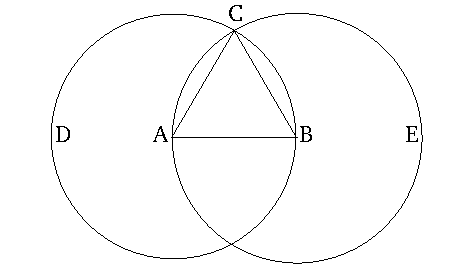
\includegraphics[scale=0.7]{circle}
%\caption{}
%\label{fig:prop 34}
%\end{figure}

%\noindent Definition of Circle: A Circle is a plane figure contained by one line, such that all of the straight-lines falling upon it from one point among those lying within the figure are equal to one another

\end{document}

